
\subsection{What is Social Weaver}\label{what_is_sowe}
Social Weaver (SoWe) is the name of a prototype system that weaves social web features into web applications. The system consists of a firefox plugin and the server side.

\begin{figure}[h!] \centering
		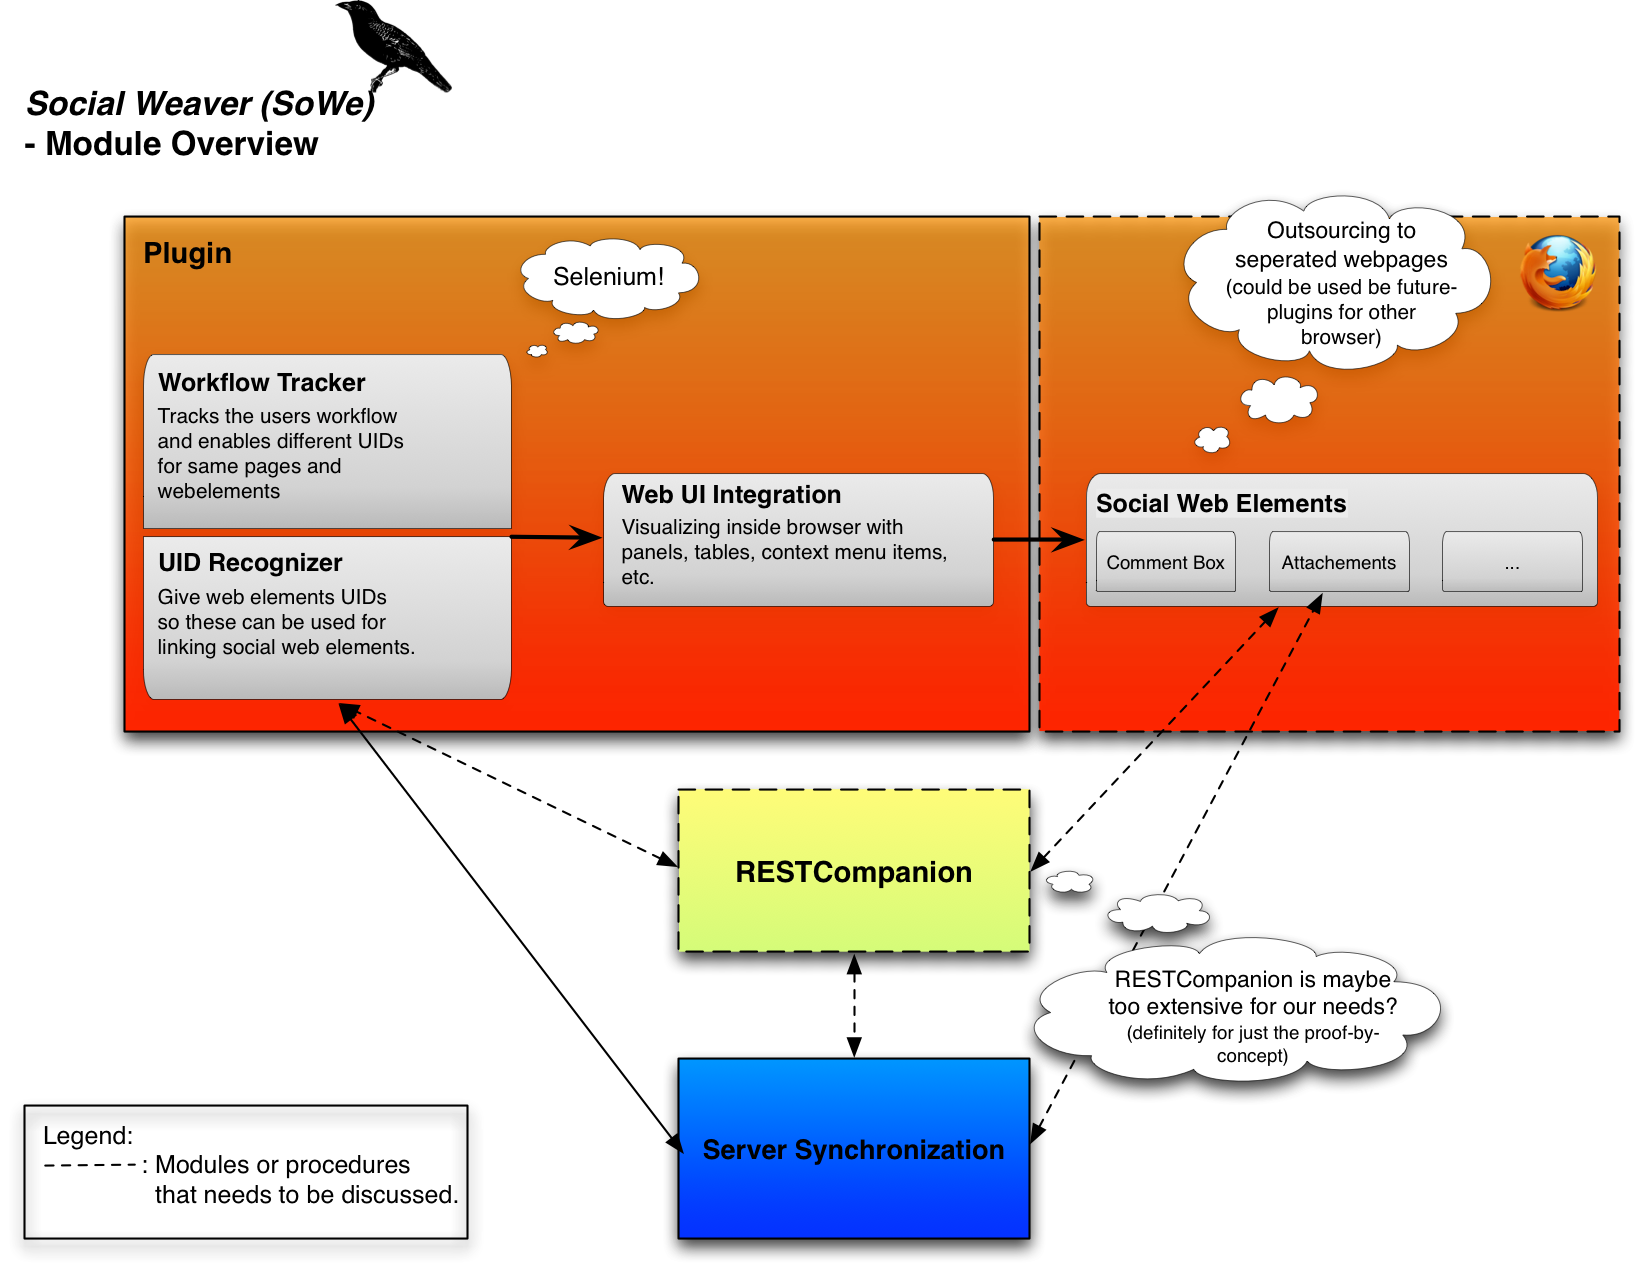
\includegraphics[width=13cm]{images/sowe-module-overview.png}
		\caption{Social Weaver Module Overview}
		\label{msowe-module-overview}
\end{figure} 

The plugin takes control of one or multiple user sessions and draws the additional content into the browser view. The server application synchronizes with each plugin and distributes updates between several clients. 

For a better understanding lets step through a generic use case where a user just opens a web application and modifies some content. The use case enumeration is related to the figure \ref{sowe-prototype-use-case}.

\begin{enumerate}
\item The user opens a web application
\item The SoWe-Plugin sends a notification to the server with all necessary information like user identifier, timestamp, ...
\item After the server receives the plugin message it synchronizes it with its current content in the database
\item The server application responses to the plugin client with content data if some exists
\item The plugin uses the content information from the server to insert all social web elements
\item The user decides to make some changes to the social web content (e.g. adds a comment or creates a new comment box)
\item Again a notification is being sent to the server with containing the changes
\item Server synchronizes the updates and responses
\item Plugin redraws the synchronized content
\end{enumerate}

\begin{figure}[h!] \centering
		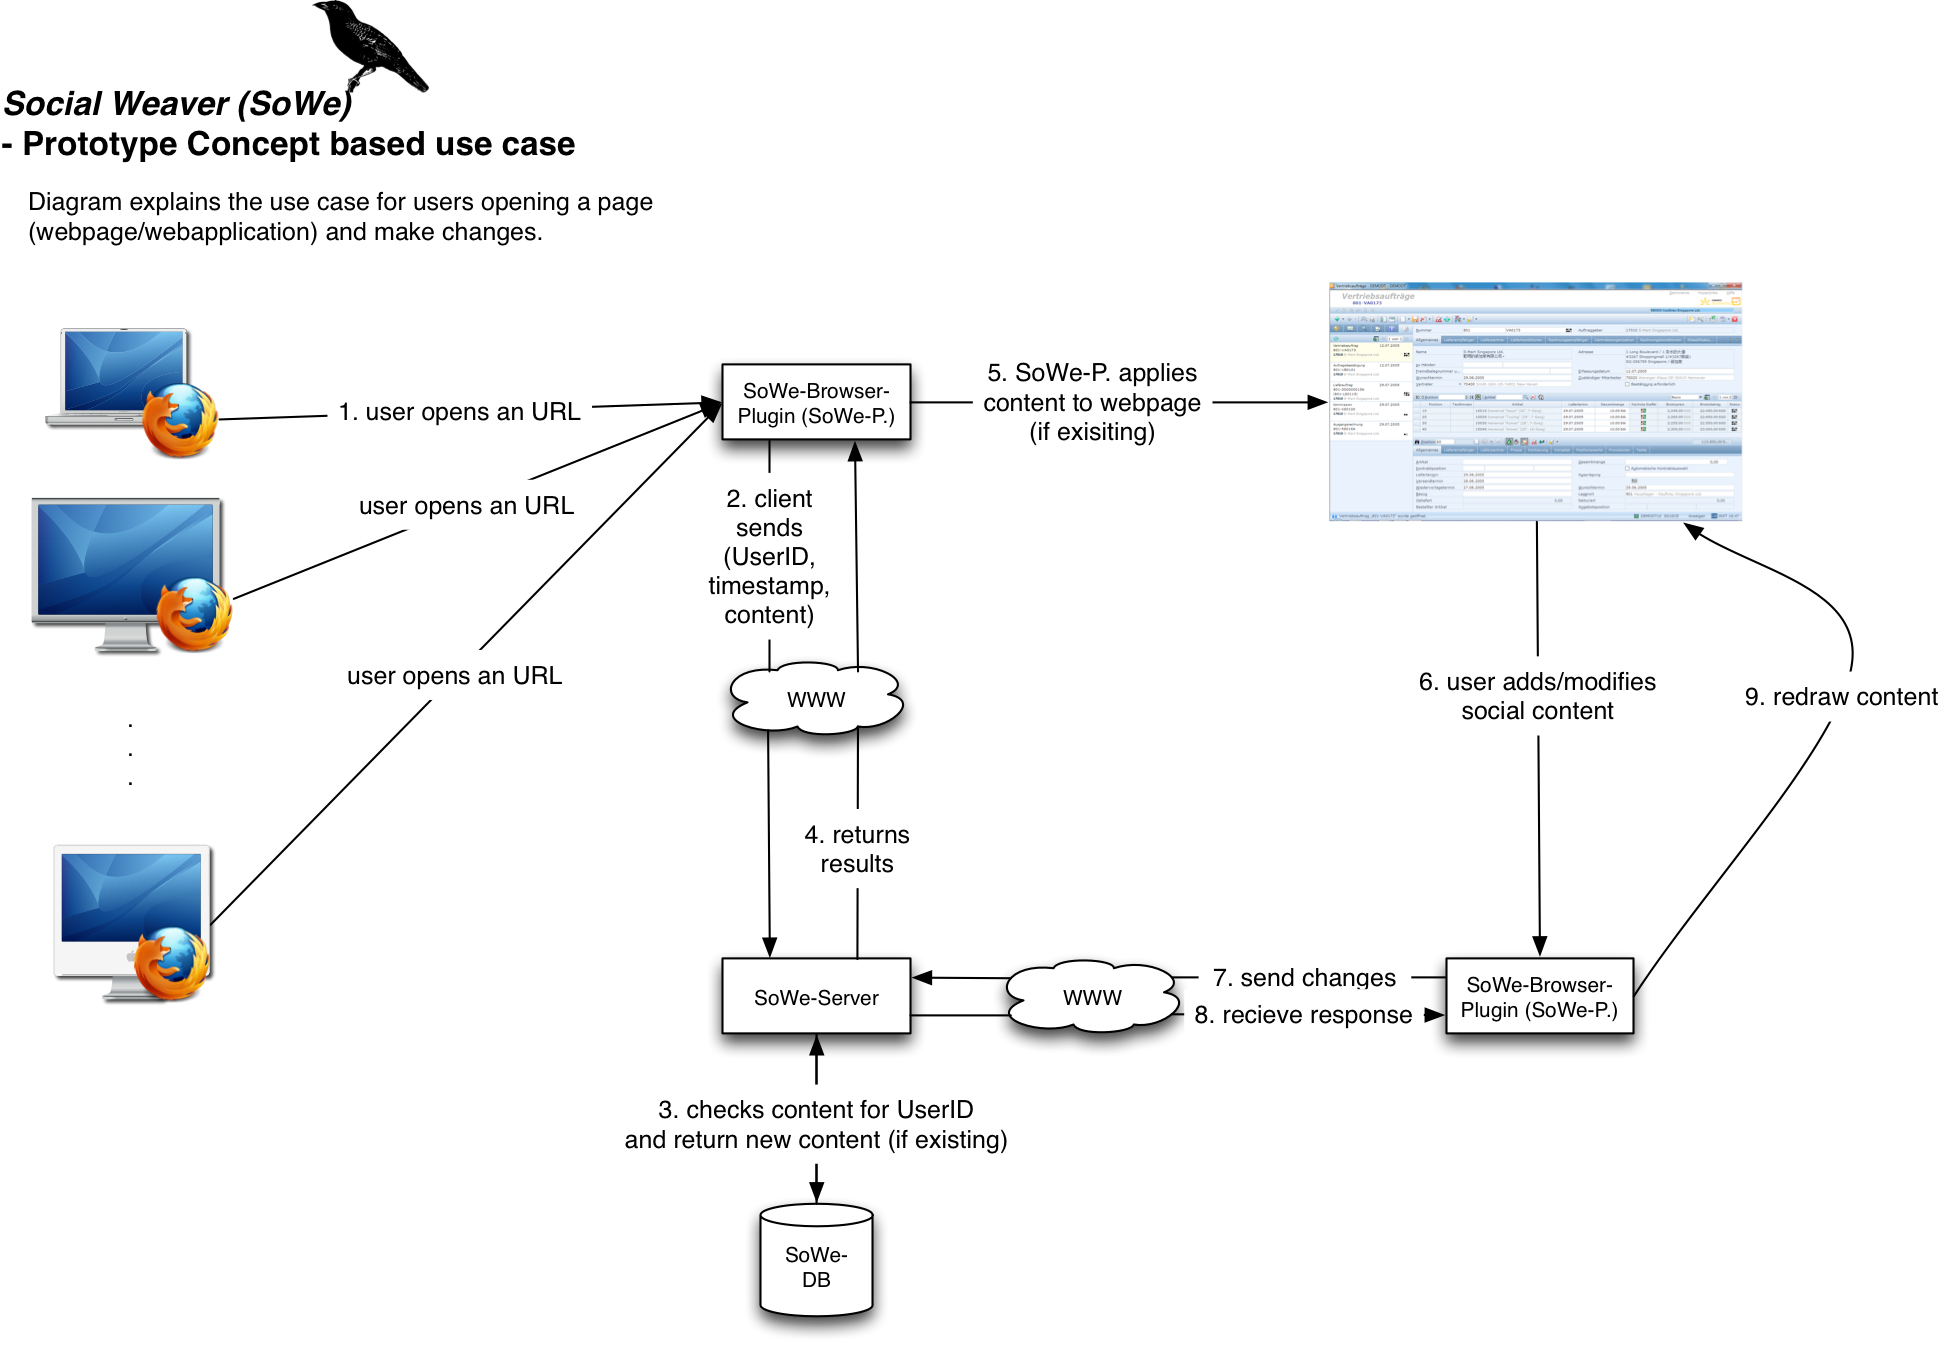
\includegraphics[width=13cm]{images/sowe-prototype-use-case.png}
		\caption{Social Weaver Prototype Use Case}
		\label{sowe-prototype-use-case}
\end{figure} 

\subsection{Requirements for Social Weaver}\label{sowe-reqs}

The general goal for Social Weaver is to weave social web 2.0 features into web-based applications. Since this is a broad requirement and impossible to be applied to any web application right from the beginning; it is necessary to break it down for the prototype.

More specifically the primary goal should be to get a system, that weaves one social web feature into a specific web application. SoWe has to be designed in a modular way, so that it will be possible to add more social media features, support multiple platforms and more web applications. Now that we have a rough idea what SoWe is going to be, lets list some concrete high-level requirements:

\begin{enumerate}
\item Browser plugin that supports a comment box
\item Server application that stores and synchronizes data that it receives from different client-plugins
\item Data format for storing and processing data for social web content
\item Communication protocol between plugin and server
\end{enumerate}

With these requirements we can start to specify our enlisting in detail:

\subsubsection{Browser Plugin}\label{browser_plugin}
In the following we define requirements on a abstract domain level according to \cite{van2009requirements}. A specification to a concrete domain level will follow in section \ref{firefox_plugin_requirements}, where we have specified what technologies to use.

As already mentioned the main requirement is that the plugin supports a comment box. That means that the browser has to display a comment box that is related to specific web element. For example in an online calendar an user adds a comment box related to an appointment that he wants to discuss in detail. 
Because it should be possible to add multiple comment boxes to any web element, we cannot just drop a box inside the user view, overlapping other interesting parts of the web application. Hence we have the requirement to make additional content visible to the user without interfering with the view on the original content. Possibilities would be fold/unfold-windows or just using small icons as references in the original view and outsource additional social content in external windows.

Of course the plugin needs to be able to communicate to the server application as well. (The server application is explained in the next section: \ref{Social Weaver - Server Application}). First of all the plugin needs to receive data that it print to the screen. Secondly changes made by the user has to be reported to the server. Because we are distributing the information between several users, there is also a need for synchronization. User updates may not overwrite updates made by other users etc.

The parser framework will contain application programming interfaces that create and parse the content of our tuples. This way it will be easier to add plugins for other browsers for instance. 
The data in the content-part of our tuple should have a uniform format no matter what web application or browser is in use. The server application will not need to know anything about the environment the plugin works in - it manages the social web content independently.

Another tricky and important point is the interaction with the web application. Most such sites are dynamic and there exists no static URLs we can refer to. And it is not certain that the same element, that two users refer to in their independent sessions, will have a comparable identifier. This issue definitely needs to be handled specifically for any web application. The good news is that this only affects the plugin. The server application just needs clearly defined identifiers. As a solution for the plugin we will need the possibility to use scripts for identifying elements. For example a script that supports the google calendar will be injected to make the plugin identify same appointments in different user sessions. This requirement is probably the vastly problematic one because it prevents a general usage of Social Weaver.

Lets summarize all the requirements we gained in this section:

\begin{enumerate}
\item Displaying and managing a comment box related to specific web element
\item Managing several comment boxes without disturbing the view on original content
\item Communication to server application
\item Creating Anchors
\item Creating content in uniform sending format
\item Parsing content from uniform sending format
\item Identifying web elements across different user sessions
\end{enumerate}

\subsubsection{Server Application} \label{Social Weaver - Server Application}
The server applications primary requirement is to synchronize different user sessions on one or multiple web applications. A user session is defined within the plugin (which does not mean a plugin can manage only one session). The server basically receives messages from different sessions, synchronizes them and distributes the most current state to all sessions.  To establish a lossless synchronization every message contains a timestamp.

We are assuming that every message contains an user identifier, a timestamp and an unique identifier for an element within the web application. This Anchor is the unique identifier for a single user action. For example if a user adds a comment to an already existing comment box that is related to an appointment in a calendar, the server receives the users identifier, the timestamp for the modification and an identifier for the appointment in the calendar. With this information the server can check its database for the comment box and add the new comment. 

It is important to remember that the server only uses the received data as identifier. All actions are completely independent to the web application. 

Also we may assume that the received message have the same Anchor form as discussed in the previous section. 
\begin{verbatim}(user identifier, timestamp, content)\end{verbatim} 
The content part from the Anchor will already be in a uniform that has been generated by the plugin. So even the browser type will not matter to the server. The server has to be able to parse the content package and to create a new one that can be parsed by our plugins.

So the requirements for the server application are:
\begin{enumerate}
\item Offer service that receives messages from plugin-clients
\item Synchronization for requests from different user-session
\item Persist updates into a database
\item Keep the server application independent to weaved-into web application
\item Parse incoming messages
\item Create outgoing messages
\end{enumerate}


%%%kommt vermutlich raus %%% \subsubsection{Communication Protocol}\label{communication_protocol}

\subsubsection{Social Weaver - Script Support} \label{abstract-script-support-reqs}
The support for external scripts is essential for a generic usage of Social Weaver. The reason why script support is extracted into its own section, is that it should be decoupled from the server and plugin that were discussen before. 

The underlying problem is the problematic identification of elements of a web view. There is simply no generic way of identifying elements in the users view across all web sites and applications. For that reason we need an extandable method to support more websites and applications. This could even mean that third-parties could support their own systems by just adding the script without the need to modify Social Weaver directly. In this section we will briefly discuss what the purpose of such scripts is in detail and what requirements we have to fulfill. 
\\ \\
The term \textit{script} in our context should contain only information that is needed by the plugin to identify an element. Let us consider the google calendar example once again. The case where we want to match the same appointment field across different user sessions brings the problem that there will be no identifier for the element itself. To the user it is obivous to identify it because of the appointment name, date and time. And those parameters could be just the information we need to extract into our script. How this will look in detail should be discussed in the concrete domain level section. 

The usage of scripts should be related to one or a set of URLs. This affects mostly the root URL of a server. But might be used for subparts of a web page or application. As example a script related to \textit{http://www.opensource.org/} will be applied to all subpages like \textit{http://opensource.org/docs/board-annotated}. 

But it might be of use to have a special matching procedure for sub pages.  In that case a script for \textit{http://opensource.org/faq} would overwrite the more general script. 

A set of URLs could be used for scripts that are applicable for many websites. 

The workflow when a script is used and when the default matching procedure that comes with the plugin is quite straightforward (see \figurename \ref{script-usage-basic}). When opening a new URL then the plugin should check whether there is a script for that case and depending on the search results proceed with the script or default matching procedure.

\begin{figure}\centering
		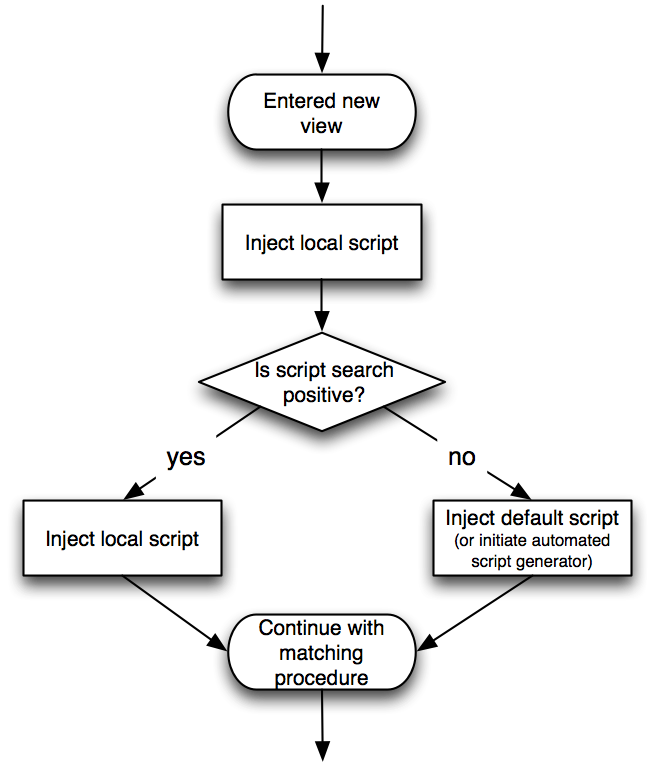
\includegraphics[width=8cm]{images/script-usage-basic.png}
		\caption{Workflow for Script Using}
		\label{script-usage-basic}
\end{figure} 

On the abstract level we will have the following requirements:

\begin{enumerate}
	\item Container of all necessary information for element matching
	\item Decoupled from browser plugin and server backend
	\item Syntax that is easy to read and write
	\item Extension of the plugin with parsing methods
	\item Default matching procedure should be provided (so the overall functionality is not limited when no scripts exist)
	\item Scripts should be related to a single or a set of URLs
\end{enumerate}
